\section{Overview}

Judas and TinyDAS are designed to process \acrshort{das} data as efficiently as possible and subsequently detect anomalies within said data. Figure \ref{fig:judasnet_overview} highlights how Judas and TinyDAS can be utilized to both process and train or analyse DAS data.

\begin{figure}[!h]
    \centering
    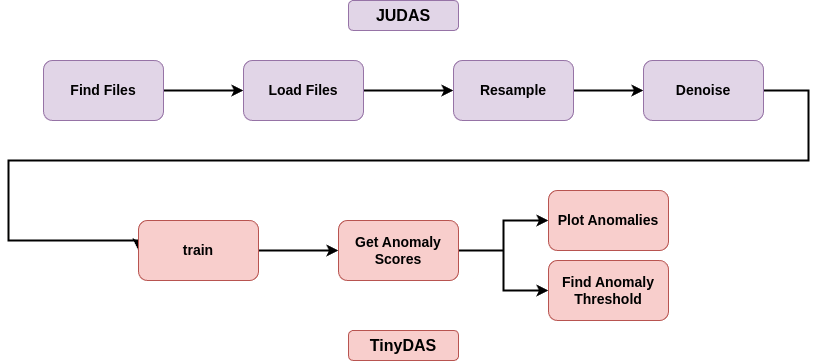
\includegraphics[scale=.4]{figures/api_overview.png}
    \caption{Judas and TinyDAS combined methodflow}
    \label{fig:judasnet_overview}
\end{figure}